\subsection{Berekening luchtweerstand}
\label{bijlage:luchtweerstand}
Een ander belangrijke eigenschap van de rover is de luchtweerstand. Deze heeft maar weinig invloed bij lage snelheden, maar begint zeker mee te tellen zodra de snelheid stijgt. Het bepalen van de luchtweerstand gebeurt in twee stappen.\\
Eerst wordt met behulp van een krachtenevenwicht (zie Figuur~\ref{image:luchtweerstand}) een differentiaalvergelijking opgesteld en opgelost. Hiermee wordt de theoretische baan van de wagen berekend. Dit staat wel nog altijd in functie van een onbekende $Cd$, de luchtweerstandsco\"effici\"ent.\\
Vervolgens wordt met behulp van video-analyse de feitelijke baan opgemeten. De werkelijke baan en de theoretische baan worden met alkaar vergeleken. Ten slotte wordt er een kleinste-kwadratische oplossing gezocht in voor $Cd$.\\
\begin{figure}[here]
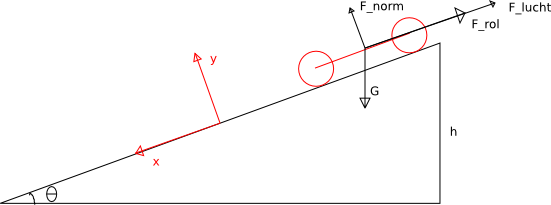
\includegraphics[width=10cm]{bijlagen/luchtweerstand/luchtweerstand.png}
\caption{Vrij-lichaamsdiagram luchtweerstand}
\label{image:luchtweerstand}
\end{figure}
\subsubsection{Theoretische baan}
%Maple file theoretische baan
Wanneer de rover naar beneden rolt, werken er vier krachten op in, namelijk de zwaartekracht, de normaalkracht, de rolweerstand en de luchtweerstand. Voor het opstellen van de bewegingsvergelijking wordt de x-as evenwijdig met de helling gelegd. Zo is de versnelling alleen maar in de x-richting en moeten alleen maar de x-componenten van de krachten beschouwd worden.
\begin{equation} \label{eq:rolweerstand}
F_{rol}=-\mu*m*g*cos(\theta)
\end{equation}
\begin{equation} \label{eq:luchtweerstand}
F_{lucht}=-\frac{1}{2}*\rho_{lucht}*A*Cd*\left(\frac{dx}{dt}\right)^2
\end{equation}
\begin{equation} \label{eq:zwaartekracht}
F_{zwaartekracht}=m*g*sin(\theta)
\end{equation}
De bewegingsvergelijking wordt dus
\begin{equation}
F_{zwaartekracht} - F{rol}-F_{lucht}=m*\left(\frac{d^2x}{dt^2}\right)^2
\end{equation}
Deze vergelijking kan opgelost worden in functie van $Cd$.
\subsubsection{Feitelijke baan}
%Excel file praktische baan
